\begin{tikzpicture}
	\node (plot) at (0,10) {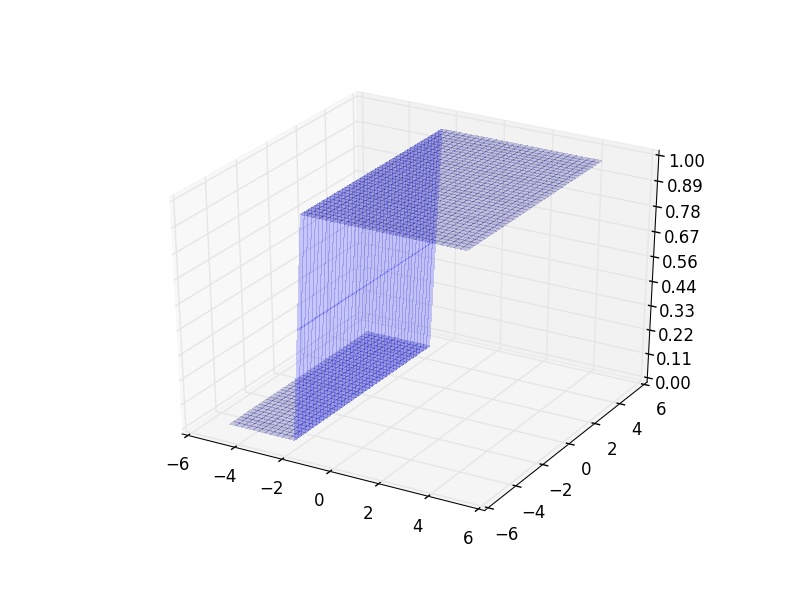
\includegraphics[width=4cm,height=4cm]{./images/module5/Plots/three/x1}};

	\node (plot) at (4,10) {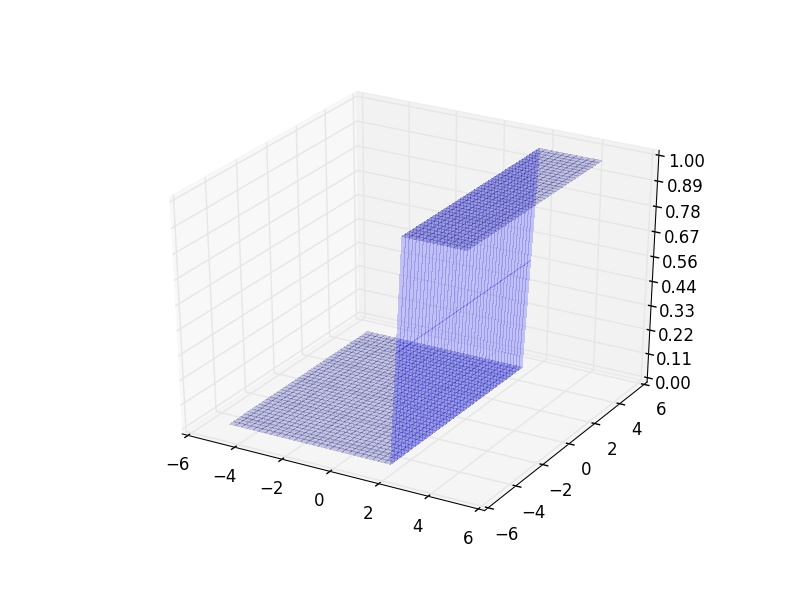
\includegraphics[width=4cm,height=4cm]{./images/module5/Plots/three/x2}};

	\onslide<3->{\node (plot) at (2,6) {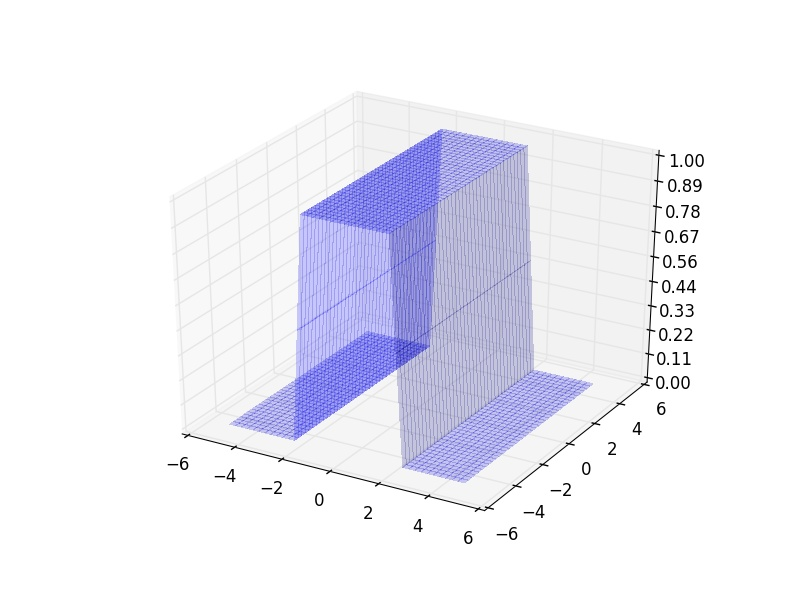
\includegraphics[width=4cm,height=4cm]{./images/module5/Plots/three/xjoin}};}
	\onslide<2->{\draw[line width=0.2mm](2, 10) -- (2.2,10);}
	%\draw[line width=0.2mm](2.1,10.1)--(2.1,9.9);
	\onslide<3->{\draw[line width=0.2mm](2,8) -- (2.2,8);}
	\onslide<3->{\draw[line width=0.2mm](2,8.1)--(2.2,8.1);}
\end{tikzpicture}